
\documentclass[british,conference,compsoc]{IEEEtran}
\usepackage[T1]{fontenc}
\usepackage{float}
\usepackage{amsmath}
\usepackage{amssymb}
\usepackage{graphicx}
\usepackage{setspace}
\usepackage{array}
\usepackage{blindtext}
%\usepackage{listings}
\usepackage{minted}
%\lstset{basicstyle=\footnotesize, language=Haskell}

\makeatletter

\newcommand{\noun}[1]{\textsc{#1}}

\@ifundefined{showcaptionsetup}{}{
 \PassOptionsToPackage{caption=false}{subfig}}
\usepackage{subfig}
\makeatother

\usepackage{babel}
\usepackage{algpseudocode}
\usepackage{algorithm}

\begin{document}

\twocolumn

\title{Plato: a tool for behavioural 
\\ specification of asynchronous circuits}
\author{Jonathan Beaumont\\
\texttt{j.r.beaumont@ncl.ac.uk}\\
\emph{School of Electrical and Electronic Engineering, Newcastle University,
UK}}

\maketitle

\begin{abstract}
Asynchronous circuits are becoming increasingly important in
system design, where they orchestrate
the interface between synchronous computation components
and the analogue environment.
However, wide adoption of asynchronous circuits by industrial users is
hindered by a steep learning curve for asynchronous control models,
such as Signal Transition Graphs, that are developed by the academic
community for specification, verification and synthesis of
asynchronous circuits.

Previously, we have introduced a novel high-level description language
for asynchronous circuits, which is based on behavioural
\textit{concepts} -- high-level descriptions of asynchronous circuit
requirements.
In this paper we will discuss our open-source tool, \noun{Plato} 
which allows the specification of asynchronous circuits using concepts, and 
features the ability to automatically translate these to Signal Transition 
Graphs for further processing by conventional asynchronous EDA 
tools, such as \noun{Petrify} and \noun{Mpsat}.
\end{abstract}

\sloppy
\thispagestyle{empty}

\vspace{-3mm}

\section{Introduction}

\vspace{-3mm}

\emph{Concepts} have been presented in order to provide a more compact
and intuitive method of designing asynchronous circuits, using a fully
compositional description method. Composition is an 
important part of concepts and the use of composition in some algebraic 
representations, such as with DI algebra~\cite{270632} and Conditional Signal 
Graphs~\cite{6243877} helped to inspire this. 

As discussed in~\cite{2015_Beaumont_MEMOCODE}, concepts are a useful language 
for specifying the behaviours of asynchronous circuits, in the preferred form 
of the user. This can be as low-level signal-level concepts, or higher-level 
gate- or protocol-level concepts. It also allows the definition of their own 
concepts, which can be reused within the same or any other specification that 
they wish to increase the speed of designing a system, and future systems. 

With concepts, we aim to solve the problems that can arise from the more 
commonly used monolithic approach with Signal Transition Graphs (STGs)~\cite{Chu_1987_phd}\cite{Rosenblum_1985_tpn},
where a user must design each system in the 
form of an STG from a blank page. The scalability of this is poor: as the 
system grows in complexity its monolithic specification becomes challenging to 
comprehend and debug. When the number of signals increases, the gates and 
protocols describing the interactions between some signals become difficult to
include with each occurance of these signals. 

\begin{figure}[h]
\vspace{-3mm}
\begin{centering}
\includegraphics[scale=0.3]{Images/cElement-stg.pdf}
\par\end{centering}
\protect\caption{\label{fig:cElement-stg} Example STG}
\vspace{-6mm}
\end{figure}

For example, Figure~\ref{fig:cElement-stg} contains an STG. 
While it seems fairly simple, and it is possible to list the interactions between each
individual signal, it would be useful to know that there is a C-element, with $a$ and $b$ as
the inputs, and $c$ as the output. Not only this, but the environment of this, what 
causes the inputs to change, is simply an inverter from the output, $c$, to both inputs. 
With this information, we have gone from listing several differing signal-level interactions,
to describing the behaviour of this circuit at gate-level. 

STGs are supported by multiple EDA tools for verification and synthesis of asynchronous control circuits,
such as \noun{Petrify}~\cite{Cortadella}, \noun{Mpsat}~\cite{khomenko2004detecting}, 
\noun{Versify}~\cite{i1997formal}, 
\noun{Workcraft}~\cite{2007_poliakov_workcraft}\cite{Workcraft_website}, 
and others. These tools take an STG specification and can formally verify its correctness, 
as well as synthesise an asynchronous circuit implementation that is 
\emph{speed-independent}, i.e. guaranteed to work correctly regardless of 
component delays~\cite{Muller_1959_ts}.

Concepts are not supported by these tools, and rather than
authoring tools to verify and synthesize concepts directly, which is a time 
consuming process, we can \emph{translate} concepts to STGs, for use with these
existing tools.

In this paper, we will discuss the implementation of the domain specific 
language and translation tool for concepts, implemented in \noun{Haskell}, called 
\noun{Plato}~\cite{2016_concepts_github}.
If STGs are the assembly language of asynchronous circuits, \noun{Plato} is a 
compiler from a higher-level language, concepts, to this assembler. \noun{Plato} is 
integrated into \noun{Workcraft}~\cite{Workcraft_website}, an open-source 
EDA tool which also features some verification and synthesis tools for STGs.

The contributions of this paper are:
\vspace{-1mm}
\begin{itemize}
  \item We detail the notations of concepts within \noun{Plato} and the built in
  concepts and their uses in Section~\ref{sec:tool-func}.
  \item We present the implemented algorithm for translating concepts to STGs
  in Section~\ref{sec:algorithm}.
  \item We explain how to use the tool from within
  \noun{Workcraft} to translate concepts in Section~\ref{sec:tool-use}.
\end{itemize}

\section{Features of \noun{Plato}\label{sec:tool-func}}

\vspace{-3mm}

The abstract base of concepts, on which these asynchronous specificications of 
circuits is discussed in~\cite{2015_Beaumont_MEMOCODE}.

\vspace{-3mm}

\subsection{Concept notation \label{sub:concept-notation}}

\vspace{-3mm}

Concepts can be composed of other concepts, and this applies to the behaviours 
of signals, as well as the specifying of the initial states and the signal 
types. This allows there to be different levels of concepts, each level of 
which will feature a composition of concepts from a lower level. 

In this section we will explain these levels, and the standard notations of 
concepts for these. 

\vspace{-2mm}

\subsubsection{\label{signal-level}Signal-level concepts}Asynchronous circuit 
specifications are mainly composed of signal transitions, and interactions 
between these, to show causal relationships. Signal transitions are denoted as 
$a^{+}$ and $a^{-}$, where $a$ is any signal name, and 
the $+$ or $-$ indicates which way the this signal transitions, $+$ denoting a 
low-to-high or 0 to 1 transition, and $-$ denoting a high-to-low, 1 to 0 
transition. 

\noun{Plato} is written in Haskell, a functional programming language. The 
domain specific language which we have implemented therefore uses Haskell 
notations, and this means some notations are different to standard signal 
transition specifications. $a^{+}$ and $a^{-}$ are in post-fix notation, where 
the operator is stated after the operand. Haskell does not support post-fix 
notation, and as such, we have to use a differing signal transition notation. 

For the tool, signal transitions $a^{+}$ and $a^{-}$ are noted as \mintinline{haskell}{rise a} and 
\mintinline{haskell}{fall a} respectively. We will use the tool notation for examples, but 
describe these using standard notation.

Signal-level concepts are the base level of concepts, and are 
the type all other concepts are built on. Here we display the standard concepts
available at this level.

A key concept in asynchronous circuits is \emph{causality}:
one signal transition \emph{causes} another signal transition, a cause and an 
effect. This is denoted in the form: 

\begin{minted}[fontsize=\normalsize]{haskell}
	    rise a ~> rise c
\end{minted}

\vspace{-1mm}

This is read as $a^{+}$ causes $c^{+}$, meaning that for the $c^{+}$ transition 
to occur, $a^{+}$ must have occurred previously. The 
\mintinline{haskell}{~>}
operator is used to show causal relationships between signals.
 
While this concept is called \emph{causality}, this doesn't necessarily imply
timings, such as any $\mathit{cause}$ transition immediately forcing the
 $\mathit{effect}$ transition it applies to. Causality can be used in order to
list all possible $\mathit{cause}$ transitions which need to occur in order
 for an $\mathit{effect}$ transition.

One can compose any concepts using the \mintinline{haskell}{<>} 
operator, and this applies
to concepts of any level, whether predefined or user-defined. For example, 
two causality concepts can be composed.

\begin{minted}[fontsize=\normalsize]{haskell}
  rise a ~> rise c <> rise b ~> rise c
\end{minted}

In words, $a^{+}$ \emph{and} $b^{+}$ must occur before $c^{+}$ can occur. 
This corresponds to so-called AND-causality in the fact that several cause 
transitions \emph{must all} have occurred before an event can occur. 
AND-causality is commonly used to imply behaviours in circuits, for specific 
requirements of effect transitions.  

The above notation can cause long-winded specifications when lots of 
AND-causality is involved. To solve this we provide a listing option. The 
following will acheive the same results:

\begin{minted}[fontsize=\normalsize]{haskell}
      [rise a, rise b] ~&~> rise c
\end{minted}

This form of concept can be composed as usual with any other concepts.

A less common, but still useful form of causality is OR-causality. This is 
where an effect transition can have several possible cause transitions. Only 
one cause transition is required to occur to allow the effect transition to 
occur. 

With OR-causality, the notation used lists all possible causes for the stated 
effect:

\begin{minted}[fontsize=\normalsize]{haskell}
      [rise x, rise y] ~|~> rise z
\end{minted}

This is, \emph{either} $x^{+}$ \emph{or} $y^{+}$ must occur in order for 
$z^{+}$ to occur. The interactions when an effect transition is included in both AND- and 
OR-causality are interesting, and an example of when this occurs can be found 
in Section~\ref{sec:algorithm}.

\vspace{-2mm}

\subsubsection{Gate-level concepts \label{subsub:gate-level}} Using the causality concept we can express
the behaviour of gates in asynchronous circuits. For example, a \emph{buffer}
is a gate with one input signal and one output signal,
whose output transitions causally depend on the input ones:

\begin{minted}[fontsize=\normalsize]{haskell}
buffer a b = rise a ~> rise b 
          <> fall a ~> fall b
\end{minted}

\noindent An \emph{inverter} has a similar conceptual specification, but the
output transition is inverted:

\begin{minted}[fontsize=\normalsize]{haskell}
inverter a b = rise a ~> fall b
            <> fall a ~> rise b
\end{minted}

\noindent A \emph{C-element} is a gate with two inputs, in this example $a$ and $b$, and one
output~$c$, which synchronises both rising and falling input transitions
via AND-causality:

\begin{minted}[fontsize=\normalsize]{haskell}
cElement a b c = rise a ~> rise c 
              <> rise b ~> rise c
              <> fall a ~> fall c 
              <> fall b ~> fall c
\end{minted}

An alternative way to express the same concept is to reuse the buffer concept:

\begin{minted}[fontsize=\normalsize]{haskell}
cElement a b c = buffer a c <> buffer b c
\end{minted}

A C-element combines the constraints imposed on the output
transitions by two `virtual' buffers. Behaviour of other gates can be similarly
defined in this way. An expanded example of a C-element and other examples can 
be found in~\cite{2015_Beaumont_MEMOCODE}.

\vspace{-2mm}

\subsubsection{Protocol-level concepts} In addition to gate-level concepts
described above it is often important to specify \emph{protocols}
of interaction between multiple gates, components or signals. Here we 
demonstrate how one can use concepts to specify asynchronous handshakes
and mutual exclusion mechanisms.

Given two signals $a$ and $b$, a \emph{handshake} between them is
the following composition of causality concepts:

\begin{minted}[fontsize=\normalsize]{haskell}
handshake a b = rise a ~> rise b 
             <> rise b ~> fall a 
             <> fall a ~> fall b 
             <> fall b ~> rise a
\end{minted}

Intuitively, we have a two-way asynchronous communication channel,
where one party sends transitions $a^{+}$ and $a^{-}$ and the other
party responds by corresponding $b^{+}$ and $b^{-}$ transitions.
Note that the four causality concepts match those found
in the buffer and inverter concepts, which leads to an alternative
way to express a handshake between~$a$ and~$b$:

\begin{minted}[fontsize=\normalsize]{haskell}
handshake a b = buffer a b <> inverter b a
\end{minted}

This conceptual understanding of a handshake as being composed
from a buffer and an inverter is often used by circuit designers as
a convenient way of reasoning.

\vspace{-2mm}

\subsection{Concepts required for translation\label{sub:trans-concepts}}

\vspace{-2mm}

The concepts we have discussed so far are aimed at specifying the behaviour of 
signals in a circuit. When translating these to STGs however, these behaviours 
do not result in a complete specification, meaning they will not be 
verifiable by standard tools, and therefore not useful in further operations, 
such as synthesis.

This is due to various parts of an STG that we have not yet discussed, which 
are important for specification, namely \emph{interface} and 
\emph{initial states}.

\vspace{-3mm}

\subsubsection{Interface concepts\label{sub:interface}} 

An important part of a specification is how these signals interact with the 
outside world, which could be another scenario or another circuit, for example.
These signals can be inputs from the outside world, outputs or an internal 
signal, which is used only within this circuit. 

To specify the type of a signal (\emph{input},
\emph{output} or \emph{internal}) we introduce the \textsf{interface} concept.
Signal types are composed according to the following rules:

\vspace{-2mm}

\[
\begin{array}{|l||l|l|l|}
\hline
\multicolumn{1}{|c||}{<>} & \mathsf{Input} & \mathsf{Output} &
\mathsf{Internal} \\ \hline \hline
\mathsf{Input} & \mathsf{Input} & \mathsf{Output} & \mathsf{Internal} \\ \hline
\mathsf{Output} & \mathsf{Output} & \mathsf{Output} & \mathsf{Internal} \\
\hline
\mathsf{Internal}& \mathsf{Internal} & \mathsf{Internal} & \mathsf{Internal} \\
\hline
\end{array}
\]

The intuition is as follows:
\begin{itemize}
    \item If a signal is an input in one component of the system, but is an
    output in another components, then in the composition it will be an output.
    \item An internal signal is similar to an output signal in the sense
that it is driven by the circuit (not the environment), but it is hidden, 
i.e. not accessible via the circuit interface. Once a signal is hidden and 
declared internal it cannot be revealed.
\end{itemize}

\noindent Specifying signal types is important when designing asynchronous
circuits, as it helps to quickly identify errors, for example, when an input transition is
caused by a hidden internal transition, as internal transitions are used only by the circuit 
and cannot be accessed from the environment, and as such, an internal transition cannot
cause an input transition. We can then reuse existing tools for circuit
simulation, verification and synthesis. Signal type information is also used
in the algorithm for automated translation of concepts to
STGs (Section~\ref{sec:algorithm}).

Concepts \textsf{inputs}, \textsf{outputs}, \textsf{internals} are defined for
specifying types of sets of signals for convenience, and to be included inline 
with other concepts. For example, to specify that signals $a$ and $b$ are 
inputs, $c$ is an output, and $t$ is internal, it is possible to write:

\begin{minted}[fontsize=\normalsize]{haskell}
inputs[a, b] <> outputs [c] <> internals [t]
\end{minted}

\vspace{-4mm}

\subsubsection{Initial state concepts\label{sub:initState}}

Specifying the initial state is important, as it determines what the first 
transitions of a scenario will be. Without these, no transition can occur.

Each signal must have it's initial state declared before translation can occur. 
In order to specify the initial state of a handshake between signals~$a$
and~$b$, we use the \mintinline{haskell}{initialise} concept.
The possible initial states are \emph{low} or \emph{high}, referred to as 
\emph{0} or \emph{1} respectively:

\begin{minted}[fontsize=\normalsize]{haskell}
    initialise a 0 <> initialise x 1
\end{minted}

\noindent A signal can only be declared as initially high or low. If the 
initial state of a signal is not defined, an error will occur, and the 
translation will not continue. Conversely, in the event a signal has it's 
initial state declared as both high and low, and is thus inconsistent, in a 
specification then the translation will also fail.

For the ease of use, and to speed up the process, initial states can also be 
declared in lists by on state:

\begin{minted}[fontsize=\normalsize]{haskell}
 initialise0[a, b, c] <> initialise1[x,y]
\end{minted}

\vspace{-1mm}

\section{Concepts to STG translation algorithm\label{sec:algorithm}}

\vspace{-2mm}

In order to reuse the tools developed by the community, it is
necessary to be able to automatically translate concept specifications to STGs.
In this section, we will display an example of how the translation algorithm 
operates, and present a pseudocode form of the algorithm in 
Algorithm~\ref{alg:translation}. 

\begin{algorithm}[t]
\begin{algorithmic}
\caption{Algorithm for translating concepts to STGs\label{alg:translation}}
\For {Signal $s$ in \textbf{System}}
  \State \textbf{define} interface of $s$ as \emph{Input/Output/Internal}
\EndFor

\For {Each effect transition $e$}
  \State $allCauses$ $\leftarrow$ Concatinate lists  possible causes for $e$
  \State $transitionList$ $\leftarrow$ \emph{Cartesian Product} \textbf{of} 
	$allCauses$
  \For {$i = 0$ to Length of $transitionList$}
    \State \textbf{add} $e(i)$ to $transitions$
  \EndFor 
\EndFor
\For {Each \textbf{signal} $s$ in system}
  \State \textbf{add} place \textbf{$s$.Name}$0$
  \State \textbf{add} place \textbf{$s$.Name}$1$
\EndFor
\For {Each \textbf{transition} $t$ in $transitions$}
  \If {transition is high}
    \State \textbf{connect} (place $t$.signalName$0$, transition)
    \State \textbf{connect} (transition, place $t$.signalName$1$)
    \For {Each \textbf{cause transition} $c$ for $t$}
      \State \textbf{read-arc} (place $t$.signalName$1$, $c$)
    \EndFor
  \EndIf
  \If {transition is low}
    \State \textbf{connect} (place $t$.signalName$1$, transition)
    \State \textbf{connect} (transition, place $t$.signalName$0$)
    \For {Each \textbf{cause transition} $c$ for $t$}
      \State \textbf{read-arc} (place $t$.signalName$0$, $c$)
    \EndFor
  \EndIf
\EndFor
\For {Each initial state $state$ concept}
  \If {$state$ is low}
    \State \textbf{add-token}(\textbf{signalName.place}$0$)
  \EndIf 
  \If {$state$ is high}
    \State \textbf{add-token}(\textbf{signalName.place}$1$)
  \EndIf
\EndFor
\end{algorithmic}
\end{algorithm}

We will use the C-element with environment example as featured in Figure~\ref{fig:cElement-stg}.
The concept specification for this will be:

\begin{minted}[fontsize=\normalsize]{haskell}
circuit a b c = operation <> interface 
             <> inits
 where
  operation = outputRise <> outputFall 
           <> inputRise <> inputFall
  outputRise = [rise a, rise b] ~&~> rise c
  outputFall = [fall a, fall b] ~&~> fall c
  inputRise = fall c ~> rise a 
           <> fall c ~> rise b
  inputFall = rise c ~> fall a 
           <> rise c ~> fall b
  interface = inputs [a, b] <> outputs [c]
  inits = initialise0 [a, b, c]
\end{minted}

This concept specification is fairly long, and describes each signal interaction.
However, we have already defined a C-element concept and an inverter concept
 in Section~\ref{subsub:gate-level}. Therefore, we can simplify this specification, 
 to use gate-level concepts instead:
 \vspace{5mm}
 
\begin{minted}[fontsize=\normalsize]{haskell}
circuit a b c = operation <> interface 
             <> inits
 where
  operation = cElement a b c 
           <> inverter c a <> inverter c b
  interface = inputs [a, b] <> outputs [c]
  inits = initialise0 [a, b, c]
\end{minted}

There can bne multiple ways of representing a specification using concepts, however,
all levels of abstraction available to the designer are built out of signal-level
concepts. Given a specification, we can therefore break down 
all gate- and protocol-level constructs into `atoms', which significantly 
simplifies the translation task. For now, we will ignore initial states and interface
concepts, and focus on the arcs only.

\begin{table}[t]
\caption{Lists of cause transitions by effect transitions
		\label{tab:list-of-concepts}}
  \centering
\begin{tabular}[htb]{| m{2.7cm} | m{2.0cm} |}
  \hline
Causes & \, Effect \\ \hline \hline
$a1^{-}$, $r2^{-}$, $a2^{-}$ 			& $r1^{+}$ 	\\ \hline
$a1^{+}$ 						& $r1^{-}$ 	\\ \hline
$r1^{+}$, $r2^{-}$, $a2^{-}$, $e^{-}$ 	& $a1^{+}$ 	\\ \hline
$r1^{-}$, $r2^{+}$, $a2^{+}$ 			& $a1^{-}$ 	\\ \hline
$a2^{-}$, $a1^{+}$, $r1^{-}$ 			& $r2^{+}$ 	\\ \hline
$a2^{+}$, $a1^{-}$, $e^{+}$ 			& $r2^{-}$ 	\\ \hline
$r2^{+}$, $a1^{+}$ 				& $a2^{+}$ 	\\ \hline
$r2^{-}$, $a1^{-}$ 				& $a2^{-}$ 	\\ \hline
$a1^{-}$ 						& $e^{+}$ 	\\ \hline
$r1^{+}$ 						& $e^{-}$	\\ \hline

  \end{tabular}
  \vspace{-3mm}
\end{table}

To start with this, we list all causes for each effect. These lists can be found in
Table~\ref{tab:list-of-concepts}.
All of the included causalities are AND-causalities, and hence, there
are several single cause transitions for each effect transition. If there were 
OR-causality included, the list of possible causes would be included with these
AND-causalities. For example:  $r2^{+}$, $a1^{+}$, $[x^{+}, y^{+}]$ causing
$a2{+}$. $x$ and $y$ are in a list of their own, and this shows OR-causalitly;
either $x$ or $y$ must transition high for $a2^{+}$ to occur. However, this does
not account for the other AND-causalities. 

In this event, we would perform the \emph{Cartesian product}, which combines
all the AND- and OR-causalities. For the example above, this would produce:

$r2^{+}$, $a1^{+}$, $x^{+}$ causes $a2/1^{+}$

$r2^{+}$, $a1^{+}$, $y^{+}$ causes $a2/2^{+}$

\noindent This includes one of the OR-causality transitions with all of the 
AND-causality transitions. It also leaves us with two separate $a2^{+}$ 
transitions. These are both needed in order to show the two possible 
combinations of transitions necessary for $a2^{+}$, and would be included as two
separate transition objects in an STG. 

However, for the David cell example, there is no OR-causality. We still perform
the step of applying the Cartesian product to each of these lists of transitions
for each effect transition, but the result will be the same as the original lists.

This concludes the part of the algorithm which defines the arcs
and transitions. Next, the algorithm begins to build the STGs. This is where
we start to use the initial state and interface concepts. 

First of all, we need to add places for each signal. These are used to
show whether a signal has transitioned high or low at any point. 
For example a token in a $0$ place shows that that signal has 
transitioned low. 

The interface is defined at the start of the algorithm, by listing them as 
$inputs$, $outputs$ or $internals$, so now we need to include all the 
transitions, and connect these to the places to form consistency loops, to 
ensure that all signals in this system can only transition in one way when this 
signal's previous transition was in the opposite direction. 

This is done by taking each transition, and if it is a $+$ transition, 
connecting the $0$ place for this signal to the transition, then connecting 
this transition to the $1$ place for this signal. Conversely, if it is a $-$ 
transition, we connect the $1$ place for this signal to the transition, and 
connect this transition to the $0$ place.

Now the algorithm introduces the initial states. All of the signals are 
specified to be initially 0, meaning that the first transition will be the $+$.
From the consistency loops, to allow this to happen, we need to place a token 
in each $0$ place for each signal.

Finally, we can add the connections to the transitions, and cause the 
expected interaction between signals. 

%We use read-arcs to connect the effect
%transitions to the places after the transition of the cause. For example, for
%\lstinline{rise a ~> rise b}, we will connect the $a1$ place to the 
%transition of $c^{+}$. We use read-arcs for these, as for this example, only
%after $c^{+}$ has occured, and placed a token in $x1$, will $c^{+}$ be allowed
%to occur, but the read arc will not consume the token in $x1$ which would block
%$x^{-}$ from being able to occur. 

Following this, the specification is fully translated, and the resulting STG 
will be the same as shown in Figure~\ref{fig:dc-stg-translated}.

\begin{figure}[h]
\vspace{-4mm}
\begin{centering}
\includegraphics[scale=0.3]{Images/dc-translated-stg}
\par\end{centering}
\protect\caption{\label{fig:dc-stg-translated} Fully translated David cell STG}
\vspace{-3mm}
\end{figure}

\vspace{-3mm}

\section{Usage of the tool\label{sec:tool-use}}

\vspace{-2mm}

%In this section, we will cover how to install the tool, how to prepare a
%concepts file and run \noun{Plato} either through command line, or through 
%\noun{Workcraft}, and the output it produces for each of these cases.

In this section, we will discuss the design flow, including the preparation of 
a concepts file, the translation methods from within \noun{Workcraft}, and 
the uses from the translated STGs. This tool can also be used from command line,
however, the design flow can include a GUI from authoring concepts to synthesis
from within \noun{Workcraft}. 

%\vspace{-2mm}
%
%\subsection{Installing the tool \label{sub:installing}}
%
%\vspace{-2mm}
%
%\noun{Plato} can be downloaded from~\cite{2016_concepts_github} on it's
%own, or it is included in the download of Workcraft. It can be used on 
%\emph{Windows}, \emph{Linux} or \emph{Mac OS X}.
%
%Download either\noun{Plato} or \noun{Workcraft}, extract it and move it to
%a known directory. Using a terminal, navigate to this directory,
%or if using \noun{Workcraft}, navigate to the \noun{Workcraft} directory, and
%then navigate to the \noun{Plato} directory, found in \texttt{tools/concepts} 
%(for \emph{OS X}, the \noun{Workcraft} directory is located within the 
%\texttt{Workcraft.app} contents folder. The concepts tool will be found at 
%\texttt{Contents/Resources/tools/concepts}.
%
%Now, the process of installing the tool is the same, regardless of how you aim 
%to use it. First of all, \noun{stack} needs to be installed 
%(download and instructions available from~\cite{stack_website}. 
%To install stack and \noun{Plato}, run: 
%
%\vspace{-2mm}
%
%\begin{lstlisting}[language=bash]
%  $ stack setup --no-system-ghc
%\end{lstlisting}
%
%\vspace{-1mm}
%
%This will prepare stack to install \noun{Plato}. Now, to build and install
%the tool, simply run:
%
%\vspace{-1mm}
%
%\begin{lstlisting}[language=bash]
%  $ stack build
%\end{lstlisting}
%
\vspace{-3mm}

\subsection{Concepts file layout \label{sub:file_layout}}

\vspace{-3mm}

\begin{figure}[h]
\begin{centering}

\begin{minted}[fontsize=\normalsize]{haskell}
module DC where

import Tuura.Concept.STG

circuit r1 a1 r2 a2 e = handshakeLeft 
                      <> handshakeRight 
                      <> outputHandshake <> interface 
	              <> initialState <> internal 
		      <> mutex <> ackHandshake 
                      <> reset
  where
  	handshakeLeft = handshake r1 a1
  	handshakeRight = handshake r2 a2
  	outputHandshake = handshake a1 r2
  	mutex = me r1 r2 
  	ackHandshake = handshake a1 a2
	reset = fall a2 ~> rise r1
  	internal = rise r1 ~> fall e 
                 <> fall e ~> rise a1 
                 <> fall a1 ~> rise e
		 <> rise e ~> fall r2
	interface = inputs[r1, a2] <> outputs[a1, r2] 
                  <> internals[e]
	initialState = initialise0 [r1, a1, r2, a2] 
                     <> initialise1 [e]
\end{minted}

\par\end{centering}
\vspace{-2mm}
\begin{centering}
\protect\caption{\label{fig:concepts_file}A concepts file}
\vspace{-2mm}
\par\end{centering}

\end{figure}

The concepts file we will discuss is found in Figure~\ref{fig:concepts_file}.
Concepts files are an extension of Haskell files, and hence, use the ``.hs'' file extension.
The following describes important information about specific lines.

\begin{description}
  \item [Line 1]  This line must be included in all concept files, with the 
  module name chosen by the user.
  
  \item [Line 2] is included so that the built-in operators and existing 
  gates/protocols can be used. 
  
  \item [Line 3] is where a user can begin to define their concepts. 
  ``\texttt{circuit}'' must begin the line for the concept to be translated.
  A user can choose what names they wish to represent their signals.
  
  \item [Line 4] is simply ``\texttt{where}''. This is used to separate the main
  concept definition from other user-defined concepts.

\end{description}

\vspace{-1mm}

The lines discussed above are the basics of writing concepts. With this 
information, a user can write concept files, but the following lines can be 
used for ease-of-use, ease-of-understanding, and reuse. 

The example we have used is of that of a David cell. We have defined the 
interface, initial state and the operation of this separatley, by defining 
these concepts following the ``\mintinline{haskell}{where}''. The full circuit 
specification is then composed of all of these defined concepts. 

\subsection{Using \noun{Plato} from within \noun{Workcraft} \label{sec:workcraft_usage}}

\vspace{-2mm}

\begin{figure*}[t]
\begin{centering}
\vspace{-3mm}
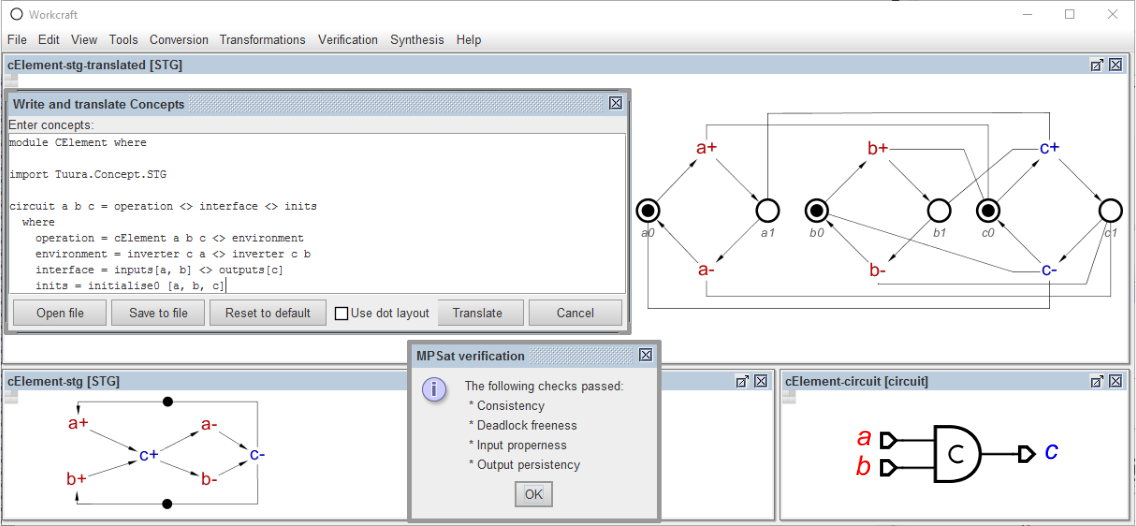
\includegraphics[scale=0.45]{Images/workcraft_design_flow.JPG}
\par\end{centering}
\begin{centering}
\protect\caption{\label{fig:design_flow_screenshot}\noun{Workcraft} and 
			\noun{plato} usage.}
\par\end{centering}
\vspace{-3mm}
\end{figure*}

\noun{Plato}, can be used on it's own using a command-line interface, and has been
integrated into \noun{Workcraft}, an open-source EDA tool. This can visualise many graphical modelling
methods, including STGs, and also features several other tools integrated, which can perform verification
and synthesis of these models automatically.

STGs are a featured modelling method within \noun{Workcraft},
which can be automatically imported from \noun{plato}, either from concept specifications written by a user from within 
\noun{Workcraft}, or by importing a previously written concept file. 
This section will discuss how to use \noun{Plato} from within
\noun{Workcraft}.

\vspace{-2mm}
 
\subsubsection{Translating and authoring concepts}

To start specifying and translating concepts, open the concepts dialog.  This is
done from the menu bar, by selecting the ``\emph{Conversion}'' menu, and then
the ``\emph{Translate concepts...}'' option. It will look similar to the dialog 
on the left in Figure~\ref{fig:design_flow_screenshot}.

From within this dialog, one can write their own concepts, from the default 
template provided. One can open an 
existing concepts file, with the \emph{.hs} extension. When satisfied with the 
concepts written, a user can choose to save the file, if not already saved, and
then translate these concepts. Translated concepts will produce an STG in a 
form similar to that on the right in Figure~\ref{fig:design_flow_screenshot}.

Now, a user can choose to insert more 
concepts, make changes to this STG, and once they are satisfied with it, can 
then perform various functions on this STG. One can perform transformations, 
verifications, simulations and synthesis on this STG using the menus within this 
workspace. Any further changes to this STG, based on the results of these 
operations can be made to this STG or to the concepts file. 

\subsubsection{Importing concepts directly}

\vspace{-2mm}

In \noun{Workcraft} it is also possible to import concepts directly from a file,
without having to view the concepts first. This can be done from the 
``\emph{File}'' menu, by selecting the ``\emph{Import...}'' option. 

\begin{figure}[H]
\begin{centering}
\vspace{-3mm}
\includegraphics[scale=0.4]{Images/import_menu_screenshot.png}
\par\end{centering}

\begin{centering}
\protect\caption{\label{fig:import_menu_screenshot}The import menu and the 
			option of \emph{.hs} files.}

\par\end{centering}
\vspace{-3mm}
\end{figure}

Any concept files imported will be automatically translated to an STG.

\vspace{-3mm}

%\subsection{Errors}
%
%\vspace{-2mm}
%
%If any errors are encountered during the translation process, \noun{Workcraft} 
%will produce a helpful error message. This usually can tell you with more 
%detail what the issue that is causing the error is, but will ask you to refer 
%to \noun{Workcraft}'s console window for specific line numbers or signals which
%need to be corrected. 
%
%These errors will include whether a signal has not been declared as an input or
%output, a signal has not had it's initial state given, or even that \noun{Plato}
%has not been installed correctly. 

\section{Conclusions and future work\label{sec:conclusions}}

\vspace{-3mm}

In this work, we have displayed the open-source
tool, \noun{Plato}~\cite{2016_concepts_github}. This tool implements a 
domain-specific language for behavioural concepts, featuring some built-in 
concepts at varying levels, allowing users to specify behaviours in a preferred 
way. 

This tool also features translation, a method of converting concepts into Signal
Transition Graphs, output in a format usable by other existing design, 
verification and synthesis tools. 

\noun{Plato}, can be used on it's own using a command-line interface, and is
integrated into \noun{Workcraft}, which can visualise many graphical modelling
methods, including STGs, which can be automatically imported from the
tool, either from concept specifications written by a user from within 
\noun{Workcraft}, or by importing a previously written concept file.
\noun{Workcraft} also features several verification and synthesis tools 
integrated, which can automatically use STGs translated from concepts. 

Using concepts, a user can reduce the time of designing an asynchronous
control circuit from the ground up, as well as allow reuse of components
by importing them from previously written user concept files which can be 
specified either as part of a scenario or entire scenarios to reduce the 
design-time of future projects. Composition of concepts can help
reduce errors and save time in comparison to performing these manually.
This method can help to make asynchronous circuits more appealing
to industrial designers.

%Currently, this method works with Signal Transition Graphs, and
%Finite State Machines~(FSM).

The \noun{Plato} tool we have discussed is available 
from~\cite{2016_concepts_github}, and as stated, is integrated into 
\noun{Workcraft}~\cite{Workcraft_website}. A manual is included with the tool, 
which features descriptions of the features. 

\bibliographystyle{unsrt}
\bibliography{publications}

\end{document}
